\section{Exercise 1 - Implement A Benchmark Framework}

The main part of task 1 was to implement a benchmarking framework for the following exercises. This was done succesfully 
and all the demanded quantities where computed and gathered in \texttt{.txt} files named with their respective
configurations and exercise number. This to postprocess and plot the data within python with low effort. 
The benchmarking framework is used in exercise 1 with a naive implementation of gathering information of all processes, 
perform an operation on the gathered information, and distribute the result of the operation to all 
participating processes. In our case we used the \texttt{MPI\_MAX} operation, which yields the largest 
element of the buffers. In the following exercises, the same idea is persued (reduce, perform operation, 
broadcast operation result) but with more sophisticated message passing approaches. \\

For all the following exercises we used bash scripts with for loops, for every exercise one bash script that
runs all the different configurations. Before compiling the C files with \fun{mpicc .. -lm -O3} one had to first run
\fun{module load mpi/openmpiS} on hydra.\\ 

For the naive implementation \texttt{MY\_Allreduce()}, which is essentially \texttt{MPI\_Reduce()} followed 
by \texttt{MPI\_Bcast()}, for powers of 10, we observed the timings shown in figure (\ref{Ex1_P10_median}).
The configurations for each graph are shown in the legend, where N is the number of Hydra Nodes, T 
the number of Processes per Node and P is e.g. powers of 10, whereby powers of 10 means that the length 
of the buffers (Count) are all powers of 10. The measurements for 36 hydra nodes and 32 tasks per node (total of 1152 \MPI 
Processes) were the slowest, while the measurement for 20 nodes and 1 task per node performed best.

\begin{figure}[h]
    \begin{center}
        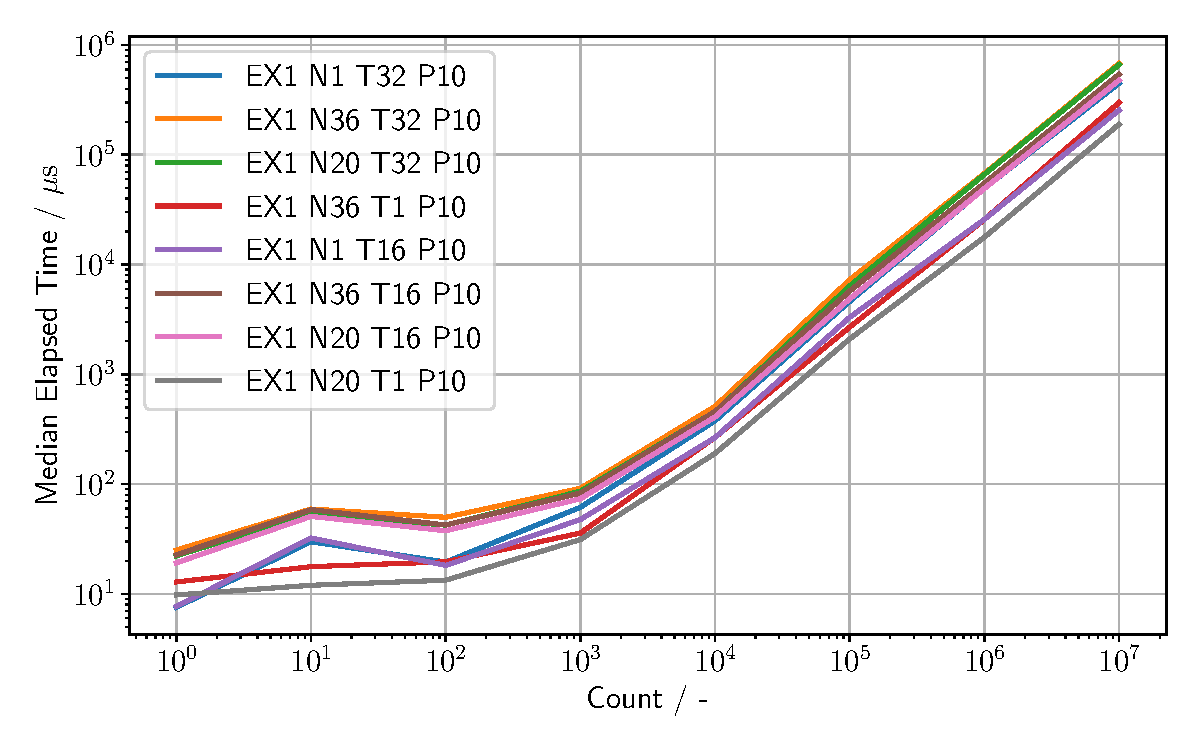
\includegraphics[width=0.8\linewidth]{figures/Ex1_1.pdf}

        \caption{Median Timings for \texttt{MPI\_Reduce + MPI\_Bcast} for all Configurations 
        and powers of 10. Since every \fun{MPI} process performs its own timing, we use 
        \fun{MPI\_Reduce(..,MPI\_MAX)} to retrieve the timing of the slowest process. After 10 Warmup rounds 
        in Ex1 we ran a 100 iterations to compute the statistical data asked for in Ex1.}

        \label{Ex1_P10_median}
    \end{center}
\end{figure}

Similar behaviour of the measurements can be observed for the ones with power of 2, see figure (\ref{Ex1_P2_median}).
Where the total highest number of \MPI processes again performed the worst and the one with 20 nodes and 1 task per 
node did the best. Also visible are jumps in all measurements except two at count = 32, the two measurements where the
jumps dont occur are the ones with only one task per node. This exact characteristics where also observed in the plot
for powers of 10, just at count = 10


\begin{figure}[h]
    \begin{center}
        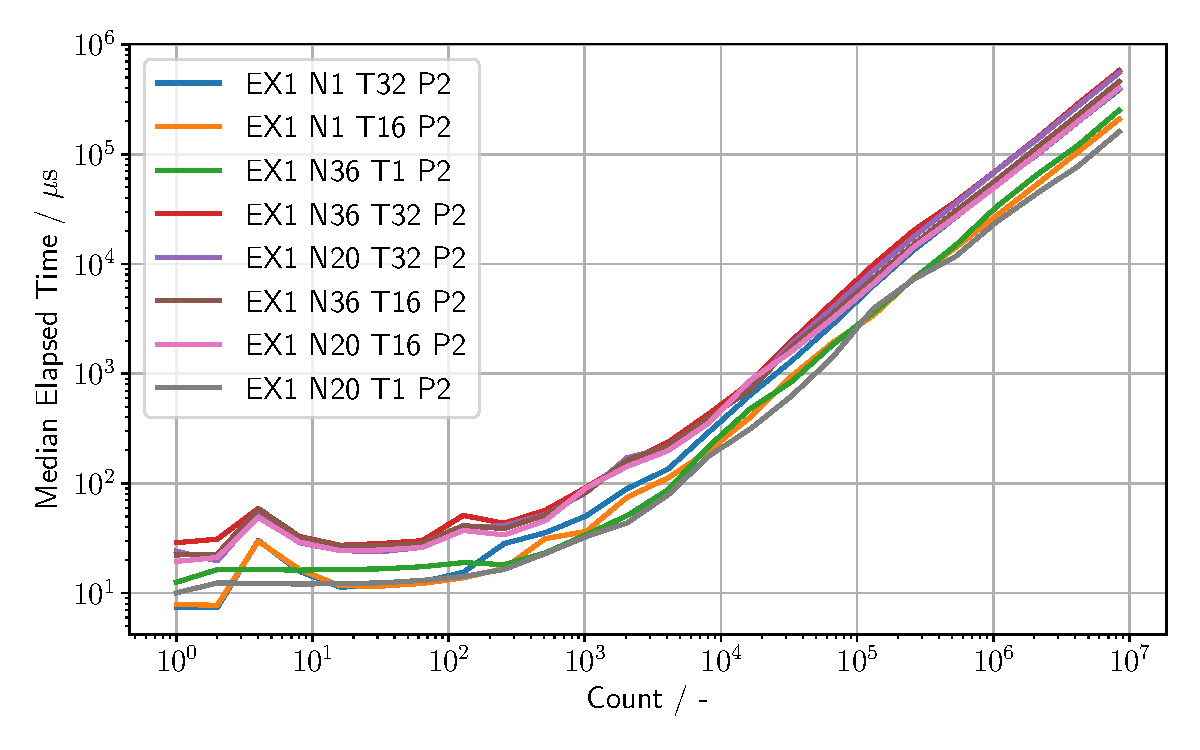
\includegraphics[width=0.8\linewidth]{figures/Ex1_2.pdf}
        \caption{Median Timings for \texttt{MPI\_Reduce + MPI\_Bcast} with all Configurations and powers of 2}
        \label{Ex1_P2_median}
    \end{center}
\end{figure}

In figure (\ref{Ex1_3_p}) we show the best and worst configurations for both powers in the same plot. 
\begin{figure}[h]
    \begin{center}
        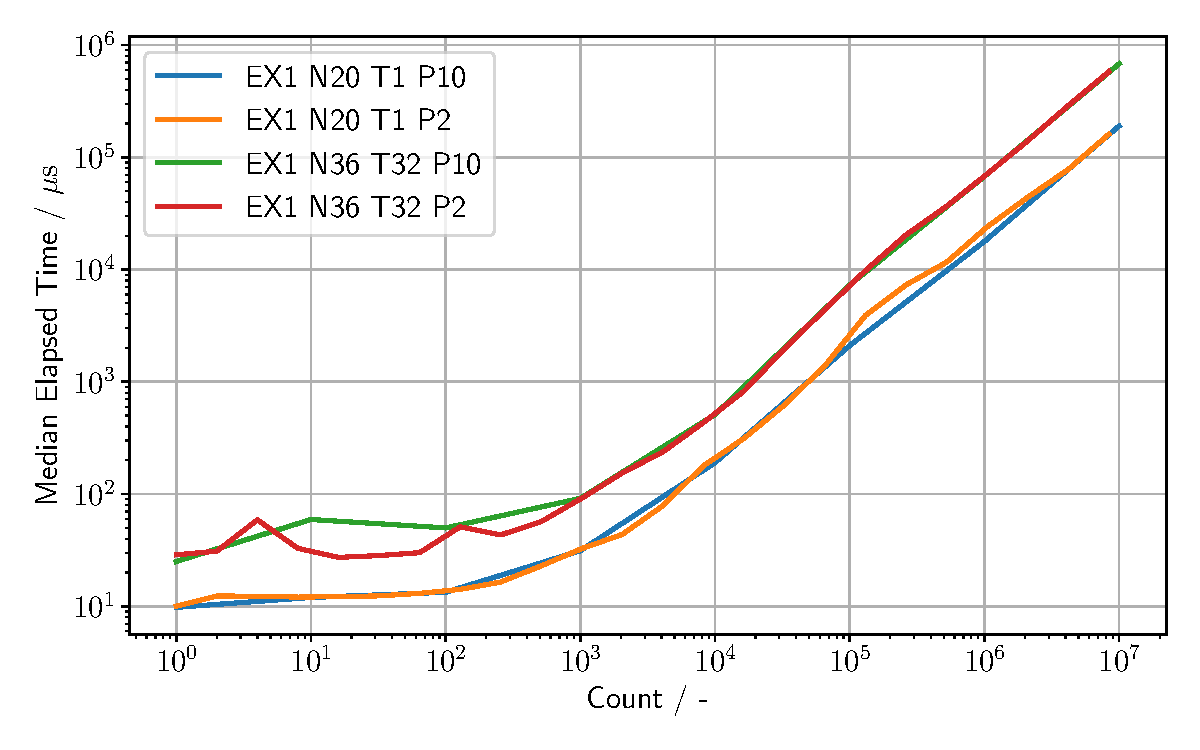
\includegraphics[width=0.8\linewidth]{figures/Ex1_3.pdf}
        \caption{Median Timings for \texttt{MPI\_Reduce + MPI\_Bcast}, best and worst configurations}
        \label{Ex1_3_p}
    \end{center}
\end{figure}

The timings shown in all figures in the document are all medians, which is an output of the statistical data postprocessing 
done in each C file to produce all the wuantities asked for in this exercise. They contain the average, median,
best seen time, standard deviation and confidence intervals.